\subsection{Оптимизация параметров алгоритмов}

При упаковки элементов в систему, а также при перемешивании элементов для генерации случайных чисел применялся алгоритм «Вихрь Мсрсенна» \cite{mersen}.

В результате исследования, основным алгоритмом для генерации случайно распределенного ансамбля выбраны алгоритмы, основанные на плотнейшей упаковке элементов. Для того, чтобы добиться равномерного распределения при различном начальном расположении элементов, следует грамотно выбирать параметры для алгоритма.

Следует учесть следующие факторы:
\begin{enumerate}
    \item Шаг $h$ для перемешивания сгенерированных элементов
    \item Количество шагов перемешивания
    \item Что является основным параметром генерации (количество элементов или плотность заполненности области генерации).
\end{enumerate}

Длина шага $h$ для перемешивания элементов выбирается на основании того, какая плотность заполненности элементов на сетке. Регулируя шаг, с которым перемешиваются элементы возможно оптимизировать количество итераций перемешивания, что позволяет добиться лучшего времени генерации. Рассмотрим на примере генерации кластера по узлам сетки. 

Также для выбора алгоритма генерации следует учесть, что если плотность элементов значительно меньше максимальной, для генерации достаточно алгоритма, основывающегося на узлах сетки.

\renewcommand{\imgsize}{8cm}
\renewcommand{\imgsubdir}{mesh_based/step_selection}
\begin{figure}[h!]
    \begin{subfigure}{0.49\textwidth}
        \centering
        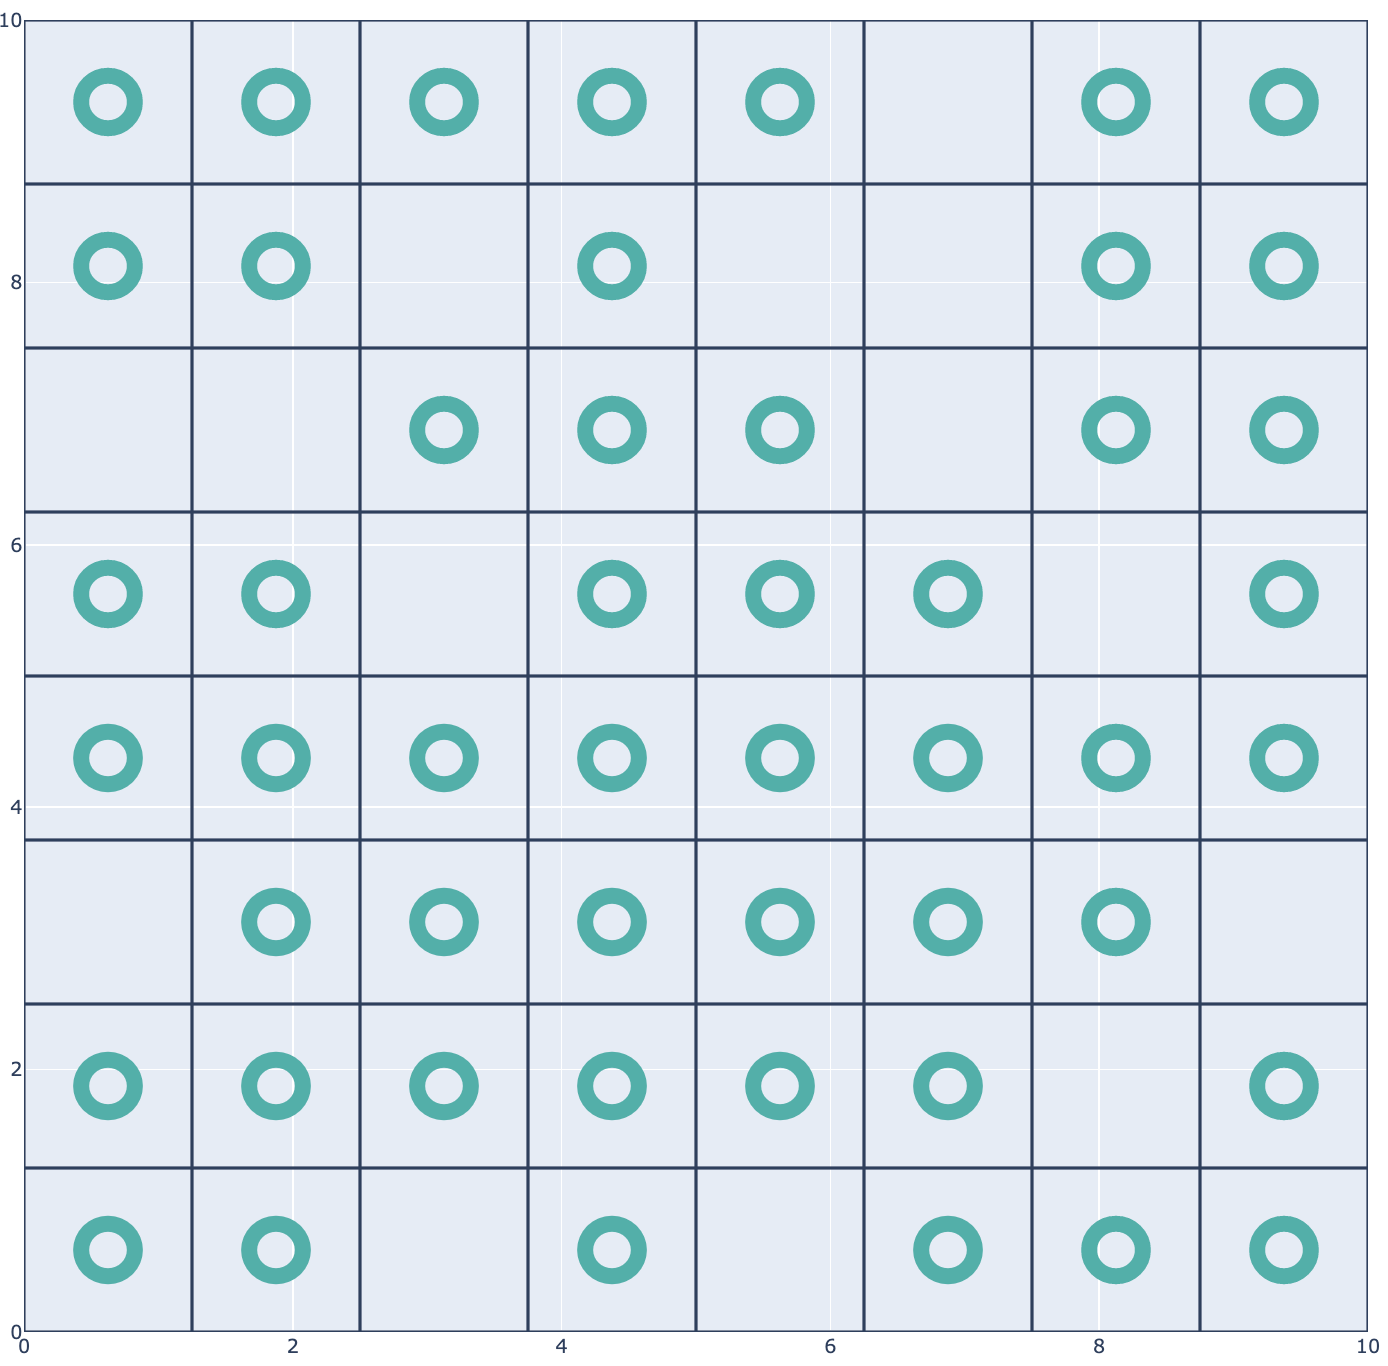
\includegraphics [width=\imgsize,height=\imgsize]
        {figures/\imgsubdir/step_selection_0.2.png}
        \caption{Плотность заполнения $6.82\%$}
    \end{subfigure}
    \begin{subfigure}{0.49\textwidth}
        \centering
        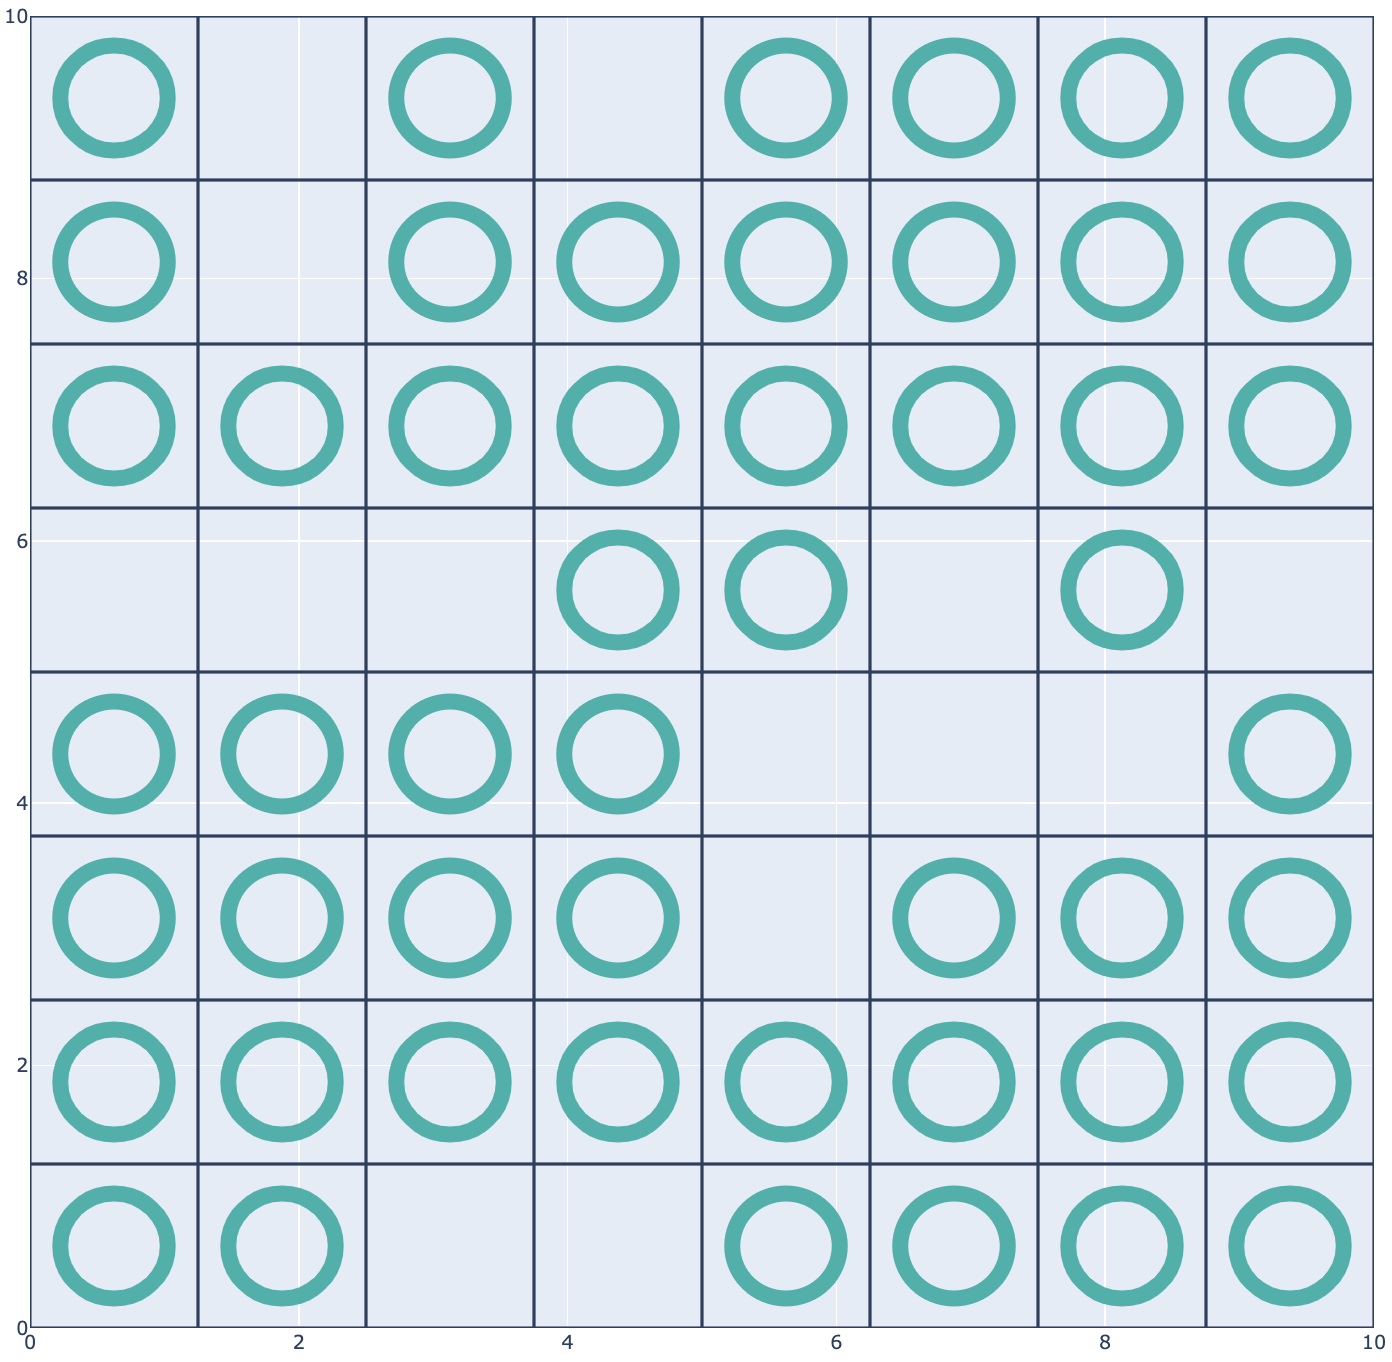
\includegraphics [width=\imgsize,height=\imgsize]
        {figures/\imgsubdir/step_selection_0.4.png}
        \caption{Плотность заполнения $25.13\%$}
    \end{subfigure}
    \caption{Расположение шаров}
    \label{fig:tight_packing}
\end{figure}

Для того, чтобы окружности были качественно и быстро перемешаны, нельзя выбирать шаг $h$ определенной, заданной заранее длины. Стандартным, для использования в подобных задачах шагом является диаметр окружности, однако когда окружности расположены друг к другу ближе, чем радиус окружности, то $90\%$ предлагаемых перемещений окружности не будут выполнены, следовательно большая вычислительная мощность будет потрачена на перемещения, которые не случатся.
В случае, когда расстояние от окружности до границы ячейки сетки, меньше, чем радиус окружности, то шаг следует выбирать как это расстояние. В ином случае, шагом следует выбирать $h$ равным диаметру окружности. 